%%%%%%%%%%%%%%%%%%%%%%%%%%%%%%%%%%%%%%%%%%%%%%%%%%%%%%%%%%%%%%%%%%%%%
% LaTeX Template: Project Titlepage Modified (v 0.1) by rcx
%
% Original Source: http://www.howtotex.com
% Date: February 2014
% 
% This is a title page template which be used for articles & reports.
% 
% This is the modified version of the original Latex template from
% aforementioned website.
% 
%%%%%%%%%%%%%%%%%%%%%%%%%%%%%%%%%%%%%%%%%%%%%%%%%%%%%%%%%%%%%%%%%%%%%%

\documentclass[12pt]{article}
\usepackage[a4paper]{geometry}
\usepackage[myheadings]{fullpage}
\usepackage{fancyhdr}
\usepackage{lastpage}
\usepackage{graphicx, wrapfig, subcaption, setspace, booktabs}
\usepackage[T1]{fontenc}
\usepackage[font=small, labelfont=bf]{caption}
\usepackage{fourier}
\usepackage[protrusion=true, expansion=true]{microtype}
\usepackage[english]{babel}
\usepackage{sectsty}
\usepackage{url, lipsum}
\usepackage[table,xcdraw]{xcolor}


\newcommand{\HRule}[1]{\rule{\linewidth}{#1}}
\onehalfspacing
\setcounter{tocdepth}{5}
\setcounter{secnumdepth}{5}
\graphicspath{ {./Images/} }

%-------------------------------------------------------------------------------
% HEADER & FOOTER
%-------------------------------------------------------------------------------
\pagestyle{fancy}
\fancyhf{}
\setlength\headheight{15pt}
\fancyhead[L]{APS490: Design Proposal}
\fancyhead[R]{University of Toronto}

%-------------------------------------------------------------------------------
% TITLE PAGE
%-------------------------------------------------------------------------------

\begin{document}
\pagenumbering{gobble}
\title{ \normalsize \textsc{APS490 - Bombardier Capstone Project}
		\\ [2.0cm]
		\HRule{0.5pt} \\
		\LARGE \textbf{\uppercase{Design Proposal}}
		\HRule{2pt} \\ [0.5cm]
		\normalsize \today \vspace*{5\baselineskip}}

\date{}

\author{
		Abhinav Ramakrishnan (999122514) \\ 
		Miaoyi Lu (998552070) \\ 
		Jonathan Ramoutar (998838003) \\ 
		Nisitha Jayatilleka (998907928) }

\maketitle
\newpage
\section*{\textsc{Executive Summary}}

The client, Bombardier Aerospace, has presented the the problem of designing a calibration block which can simulate cracks in fuselage skin and doublers (in various repair configurations). The previous report submitted dealt with the scoping of the project, identification of the stakeholders, identification of the functions, constraints, and objectives to be met by the product. The team incorporated feedback given on that report and used it to introduce the methodology, the research and the approach to the design solutions created.

Various design considerations were analyzed during the initial research phase. A broad spectrum of suitable machining tools/methods, methods for the creation of cracks, and manufacturing of skin layer and doublers, were recognized. For creation of the cracks existing methods such as laser cutting, electric discharge wire cutting, and PAN etching were explored, and an alternate approach to the method of crack creation through pressing of two plates was introduced. It is important to note that the current plate defect creation method used in the industry is the electric discharge wire cutting method. Next, methods of CNC machining and chemical milling were looked at. Furthermore, application of a gel during the assembly for the purpose of getting greater depth probing was considered.

Based on the research conducted and taking into account the above considerations, three designs were proposed. `The Staircase' design constitutes of having discrete thicknesses of the skin layer and the doubler mounted, each mounted on top of each other by rivets. This design can simulate 21 instances configurations with detectable cracks. `The Hook' design is an expansion of the idea that a crack can be simulated by pressing two plates together. It showcases how the plates can brought together such that the crack has a finite length. `The Petri Dish' is a design where a series of skin layers and doubler layers can be stacked on top of each other to create a versatile system that can replicate different thicknesses without compromising too much signal strength. The advantages and disadvantages of applying a conductive gel between the layers of skin and doublers were recognized here.

Finally, the constraints and objectives recognized and prioritized in the previous report are given a normalized grading system. It is seen that low cost and reliability are the high priority objectives the design should meet. Utilizing these weights in a weighted sum model, a rigorous analysis was done in order to compare the designs to each other and against the objectives. After the analysis, it was found that the Staircase design is the optimal design to be implemented.

\newpage

\renewcommand{\contentsname}{\textsc{Contents}}
\newpage
\textsc{\tableofcontents}
\newpage

%-------------------------------------------------------------------------------
% Section title formatting
\sectionfont{\scshape}
%-------------------------------------------------------------------------------

%-------------------------------------------------------------------------------
% BODY
%-------------------------------------------------------------------------------

\pagenumbering{arabic}
\fancyfoot[R]{Page \thepage\ of \pageref{LastPage}}
\section{Introduction}
%\addcontentsline{toc}{chapter}{Problem Statement}
The team has been asked by engineers at Bombardier Aerospace to create a design for a universal calibration block to be used in the Non-Destructive Testing of certain aircraft repair procedures. After submitting the project requirements to the clients the team received feedback that helped further define the parameters of the project and clarify the functionality, objectives, and constraints of the design.

The most notable change is that the requested calibration block need not cover 90\% of all feasible repair configurations. The client has indicated that 50\% is satisfactory. They have also requested that the solution should focus on sub-surface inspections. The design must calibrate for the detection of cracks in components covered by other material, as is the case with repair-doublers on fuselage skin. As well, the clients at Bombardier requested that Aircraft Maintenance and Manufacturing (AM\& M) as a stakeholder be changed to the Canadian General Standards Board (CGSB), since Non-Destructive Testing is more directly regulated by the CGSB. Other changes include clarification of the scope: for example, the problem is not related to fatigue analysis. Fatigue, as the client points out, pertains to the initiation of cracks - the problem at hand relates more to fracture mechanics analysis. Finally, the client has informed that traceability be specifically addressed via the inclusion of part numbers and serial numbers.

Using the feedback provided by clients and further research on NDT and calibration blocks for eddy-current, the team was able to determine how to approach the design process. Section 2 identifies the parameters the team has used for creating the necessary aspects of the designs. It also compares these parameters against the refined constraints of the project scope. Section 3 lists and describes design alternatives and possible solutions to achieve the design goals. Section 4 provides an explanation of the methods with which the design alternatives are evaluated and how they meet the requirements. Section 5 is a summary of the final proposed design.

\section{Design Considerations}
%\addcontentsline{toc}{chapter}{Background}
\subsection{\textsc{Design requirements}} 

The final product is expected to simulate at least 50\% of the repair configurations. These configurations include; fuselage-skin and repair doubler atop the fuselage, repairs near the aft baggage door, and repairs near the window and the door cutout of the `Dash-8' planes (the Q100, 200, and 300 series, as well as the Q400 series). The repair configurations can also vary according to rivet size and type, crack location, repair location, and the inclusion of structural elements such as stringers and frames. 

It was decided that for the purposes of creating the design alternatives, it is better to at first consider a broad variety of available options of design aspects, rather than focus on individual designs. This would help the team understand the industry as well as the manufacturing processes involved in these options. 

 
\subsection{\textsc{Crack creation or manufacturing of cracks}}

Ideas and available methods regarding the manufacturing of cracks will be discussed in this section. These are not the only options available, however other methods have been disregarded as they have been deemed unfeasible. For example, it is possible to create notches in a part and actually fatigue it until a crack is created - however, the costs of accomplishing this are much greater than for the methods below.

\subsubsection{Laser Cutting}
A highly focused laser beam is directed at the metal piece. This will effectively melt and evaporate the metal. This method gives relatively smooth crack walls. Laser beam cutting has an accuracy of around $\pm$0.025 mm and can cut into 6.35 mm mild steel. The width of the crack can be adjusted by focusing the beam. As the accuracy required to simulate the cracks is around 0.004 inches (0.1 mm), and the depth of crack does not exceed 1 mm, laser cutting is a viable means of generating out the cracks.

\subsubsection{Electric Discharge Wire-Cutting}
This is a variation of Electronic Discharge Machining (EDM). Here a high current is passed through a wire which is in turn used to cut through the part. The part itself is mounted on a milling machine. As the part is maneuvered the wire cuts through the metal. The accuracy of this method is comparable to that of laser cutting and is around $\pm$0.025 mm.The crack walls are similarly smooth when compared to laser cutting. The average cost of creating a notch using EDM is approximately \$75 .

\subsubsection{Aluminum PAN etching}
Theoretically it is possible to place a positive photo-resist on the aluminum part (thereby covering it completely) and then expose it using UV photo-lithography [1]. This generates a pattern on the surface of the photo-resist after it is washed with the requisite solvent. After generating the pattern we may then use an aluminum PAN solution to etch the pattern onto the surface of the part. The PAN etch does not typically have any noticeable effect on the photo-resist. The time submerged in the PAN etch decides the depth of the pattern [2]. The accuracy of this method is on the order of a hundred nano-meters (the wavelength of the light used). The cost of this method is usually around \$160 for creating the mask and approximately \$40 to acquire the materials for the photo-resist and the PAN solution. The price does not change significantly with the number of cracks to be generated since all these processes can be done in batches. The cost of using the machines involved is dependent on the number of hours of machining - at the University of Toronto the cost is \$32 per hour of use (capped at \$350 per month).

\subsubsection{Adjacent sheets}
Pushing two metal sheets of equal thickness together is a way of simulating a finer crack than by machining. The length of the crack simulated is then equal to the length of contact between the two sheets. This means that creating cracks within a layer of metal - that are not edge cracks or that do not cleave the layer completely - is difficult. Section 3.2 provides a possible solution to this. This method is still useful in that it does not include any additional costs beyond the machining of the plate geometries.


\subsection{\textsc{Fabrication of the Calibration Block}}
Manufacturing and assembly methods for the calibration blocks will be discussed here. These methods address the means of creating the metal plates that represent the fuselage skin, repair doublers, and the various thicknesses of both.  Special consideration is given to the surface quality of the machined parts, and the accuracy of the machining method. 

\subsubsection{Computer Numerical Control (CNC milling machine)}
CNC machining is one of the most popular types of machining in the industry. Fundamentally this can be described as a computer guided milling process. Due to the application of an automated control system, most human errors and inaccuracies that occur during manual machining are avoided. CNC machining provides a fast and accurate method of machining. The total machining costs have been estimated to be upwards of \$200 [3].  

\subsubsection{Chemical milling}
This method uses baths of etching chemicals to create a necessary shape. A corrosive chemical reagent called an `etchant' is applied over the areas where the material needs to be removed. The etchant reacts with the material and dissolves the surface. Inert chemicals are applied over non-etch surfaces [4].

\subsubsection{Gel/Tape Adhesion}
A simulation of one thickness of material can be created by joining together many thinner sheets by placing one on top of the other, hence totaling up to the required thickness. However there exist air gaps between the thinner layers which reduce the probing depth and amplitude of the eddy current, weakening the signal being read. As a solution, a gel/tape with comparable conductivity to the material of the block itself is suggested for application between the layers. In other words, in lieu of an air interface there is now a gel/tape interface. Section 3.3 expands on this method with a design dubbed `Petri Dish'.

\section{Alternative Designs}
%\addcontentsline{toc}{chapter}{Stakeholders}
The following alternative designs were created upon consideration of the processes described in Section 2. Deciding on processes that are cheaper and simpler to implement the team was then able to create the following three alternatives. Each one expands on a different method and combines methods of crack creation and varying thickness.

The design will be made of an aluminum alloy. 2024-T3 aluminum alloy is used for skin and repair doublers.

`The Staircase' and `The Petri Dish' are the chosen names for two alternatives for generating various thickness; photo-lithography (using PAN etching), EDM, and laser cutting are three cutting technologies that can be used to simulate cracks on any design. `The Hook' is a third design which is based on tightly pushing plates together. It doesn't require any cutting technologies but still allows for finite crack length. 

\subsection{\textsc{The Staircase} }

\begin{figure}[h!]
  \centering
  	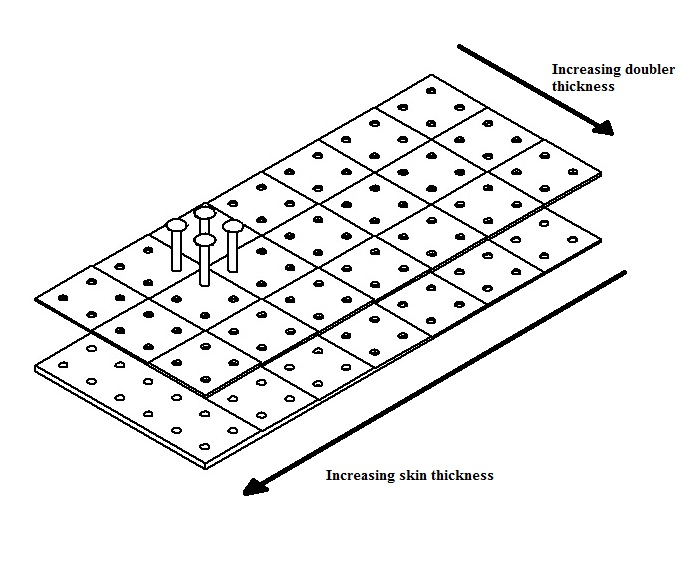
\includegraphics[width=\textwidth]{Steps_iso}
  \caption{Isometric exploded assembly view of `The Staircase'}
  \label{fig:steps_iso}
\end{figure}

\begin{figure}[h!]
  \centering
  	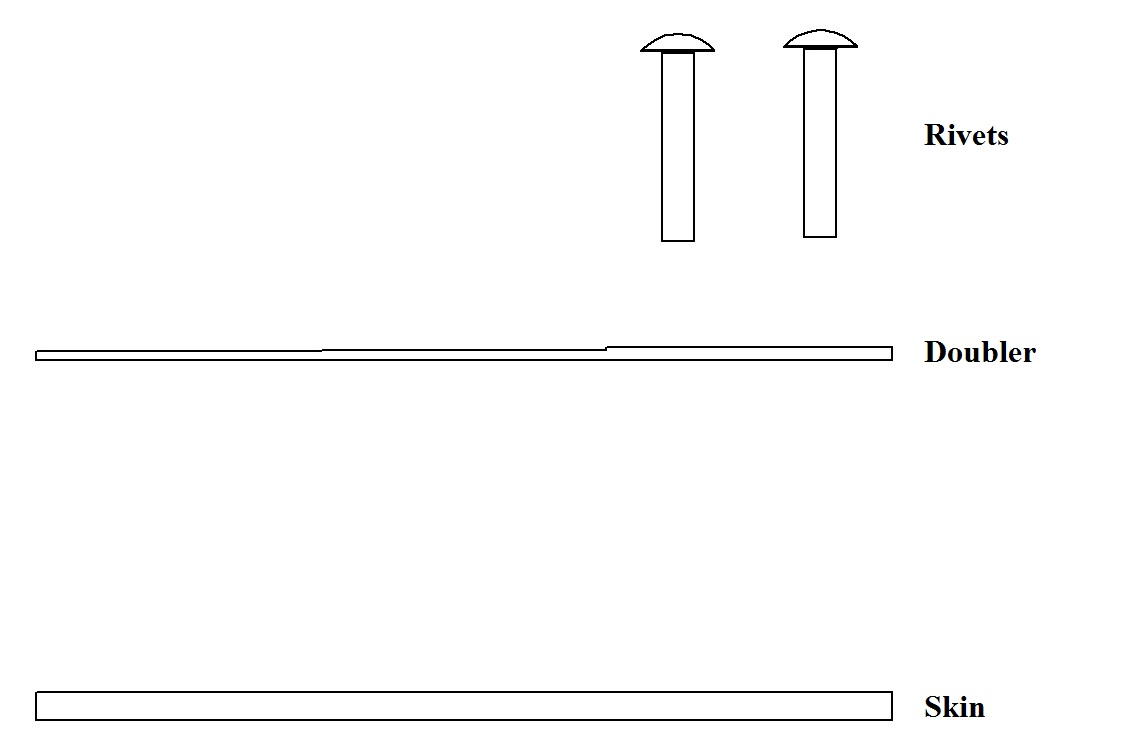
\includegraphics[width=\textwidth]{Steps_front}
  \caption{Front exploded assembly view of `The Staircase'}
  \label{fig:steps_front}
\end{figure}

\begin{figure}[h!]
  \centering
  	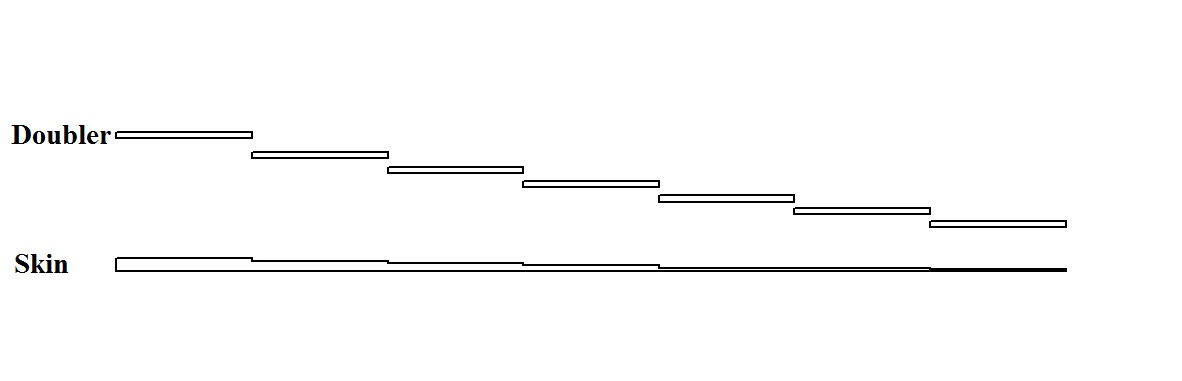
\includegraphics[width=\textwidth]{Steps_right}
  \caption{Right exploded assembly view of `The Staircase'}
  \label{fig:steps_right}
\end{figure}

The staircase design is composed of three major portions;  fuselage skin as a whole with varying thickness,  repair-doubler plates with various thicknesses, and rivets to fasten each repair-doubler plate onto the fuselage skin. The directions of thickness variance is shown in Fig. \ref{fig:steps_iso}.

The fuselage skin is machined from a single block of aluminum. The thickness varies in 7 discrete steps. 12 rivet holes are drilled into each such step as shown in the figure. Cracks can be simulated between two rivets (or a rivet pitch). Each thickness combination has one edge crack propagating from the edge of the body. The skin layer thicknesses can be CNC milled or chemical milled. Other machining methods available are considered too expensive.

As shown in Fig.\ref{fig:steps_right}, the doublers are emulated by 7 separate identical plates with 3 different thicknesses. Each is fastened onto every stair step of the fuselage skin. Hence, one individual plate simulates three doubler thicknesses along one skin thickness.

In conclusion, the aspect of generating various thicknesses is solved in this design by fastening two staircases perpendicular to each other, which creates a total of 21 (3x7) configurations. Cracks can be created on the fuselage skin through laser cutting or EDM.
\clearpage
\subsection{\textsc{The Hook} }

\begin{figure}[h!]
  \centering
  	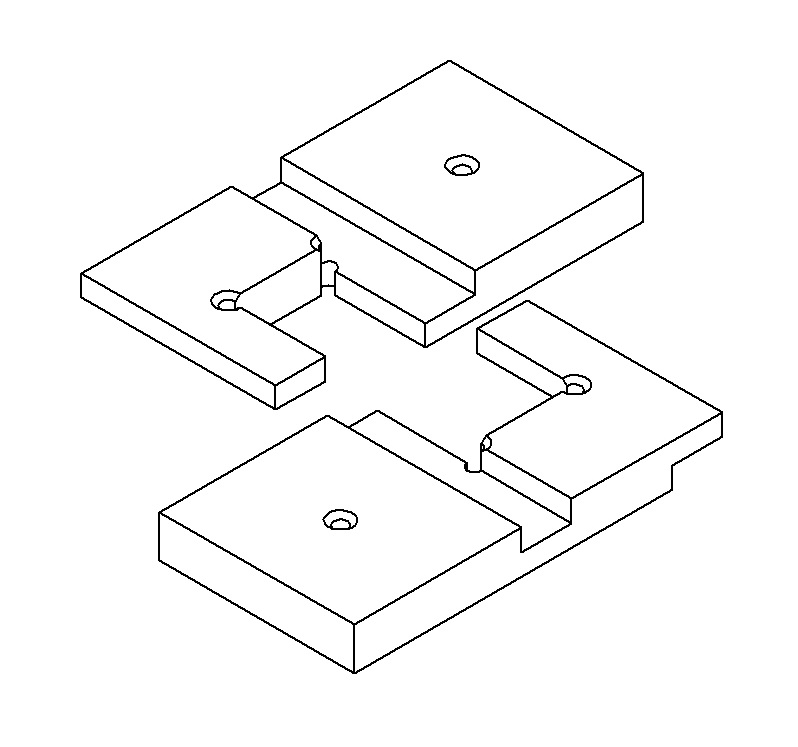
\includegraphics[width=\textwidth]{Hook_iso}
  \caption{Isometric exploded assembly view of proof-of-concept of `The Hook'}
  \label{fig:hook_iso}
\end{figure}

\begin{figure}[h!]
  \centering
  	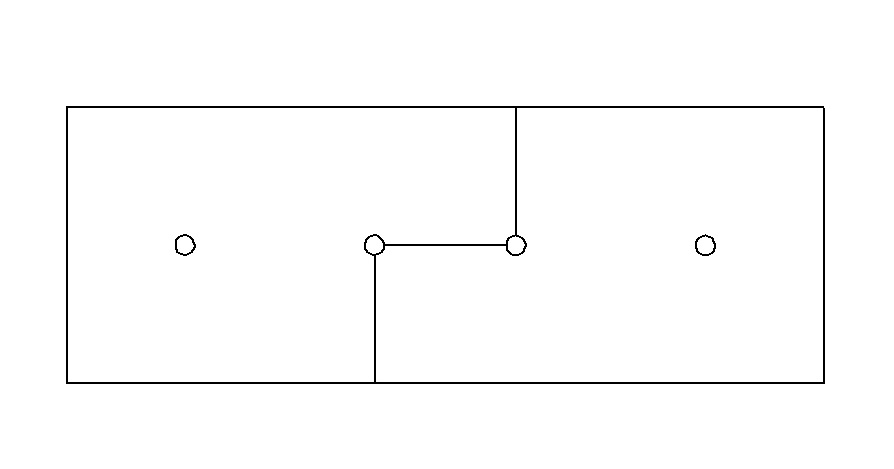
\includegraphics[width=\textwidth]{Hook_top}
  \caption{Top assembly view of proof-of-concept of `The Hook'}
  \label{fig:hook_top}
\end{figure}

\begin{figure}[h!]
  \centering
  	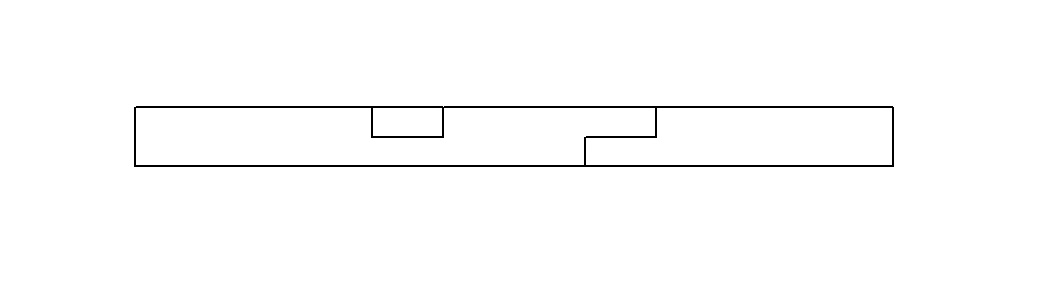
\includegraphics[width=\textwidth]{Hook_right}
  \caption{Right assembly view of proof-of-concept of `The Hook'}
  \label{fig:hook_right}
\end{figure}

The focus of the `The Hook' design is the creation of a fine crack by pushing two plates together. Normally, even though this method yields great results in crack width, the cracks themselves are technically infinitely long (see section 2.3). The Hook design attempts to rectify this issue by using two plates with geometry that allows them to be slotted together. Fig.\ref{fig:hook_iso} roughly shows the concept of such slotting. Once connected, the two pieces form one single layer (the fuselage skin). Fig.\ref{fig:hook_top} shows a portion of such a layer, demonstrating how the crack created would be between two rivets. Additional rivets may be added to each hook piece to provide balance points - while only two more are shown a final design would incorporate more. This assembled layer would be riveted to another sheet (say, a doubler) (not pictured), replicating the repair configuration and keeping the slotted pieces together.

Fig.\ref{fig:hook_right} shows how the thickness of a layer is constant along the length of the crack, and beyond the edge of each slot. In between, though, there is a discontinuity where the two pieces connect vertically. This is a considerable downside as it may affect the signal in unwanted ways.

There would be two hooks per skin layer thickness. Doublers of different thicknesses may interchangeably be fastened to these hooked skin layers. Though only one row of rivets has been shown in the figures, those figures are only an illustration of the slot mechanism; multiple rows of rivets may be incorporated with only minimal change to the geometry.

\clearpage
\subsection{\textsc{The Petri Dish} }

\begin{figure}[h!]
  \centering
  	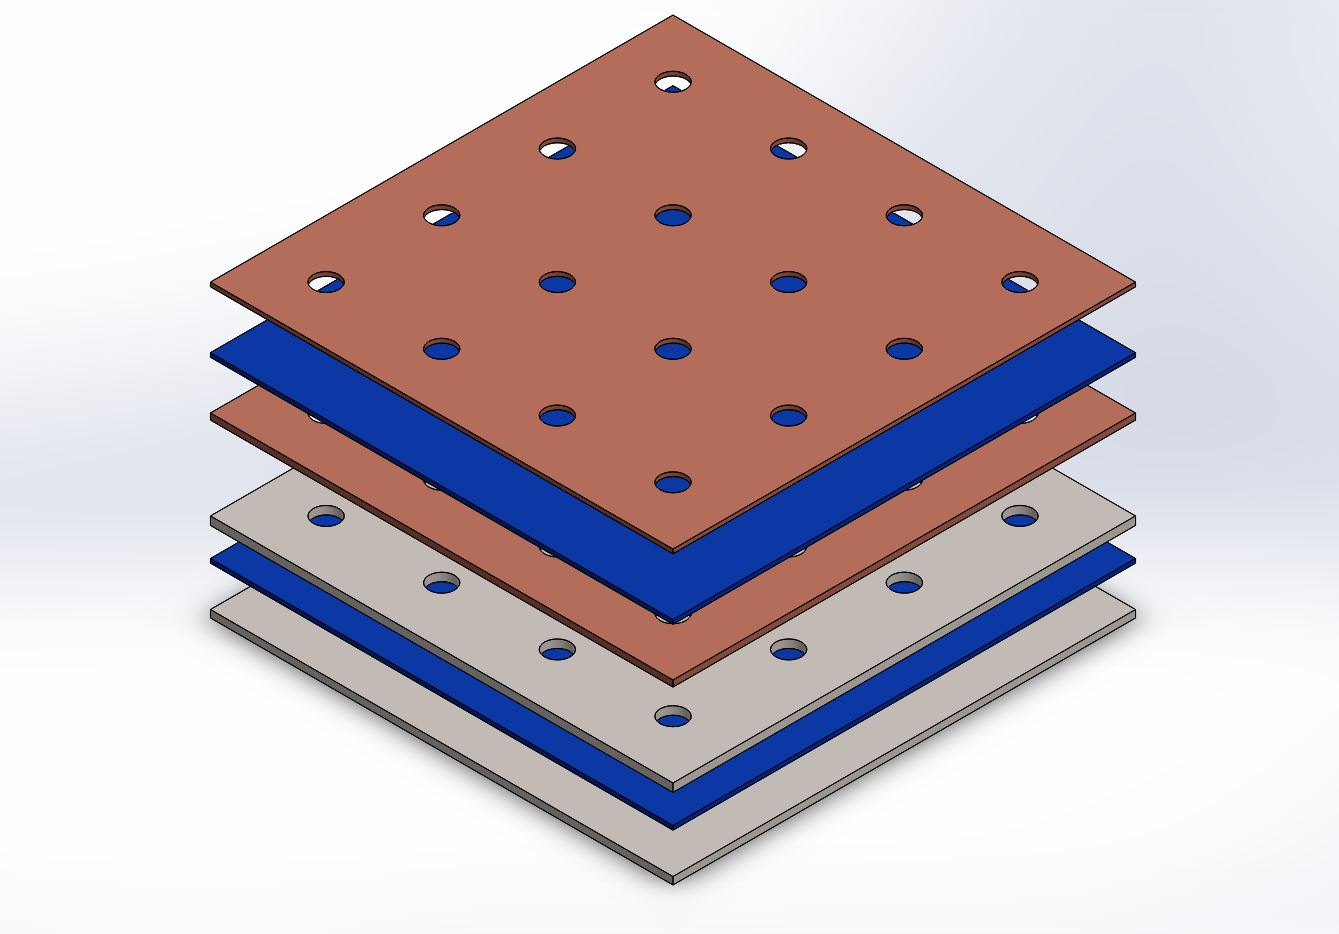
\includegraphics[width=\textwidth]{Petri_iso}
  \caption{Right assembly view of proof-of-concept of `The Petri Dish'}
  \label{fig:petri_iso}
\end{figure}

\begin{figure}[h!]
  \centering
  	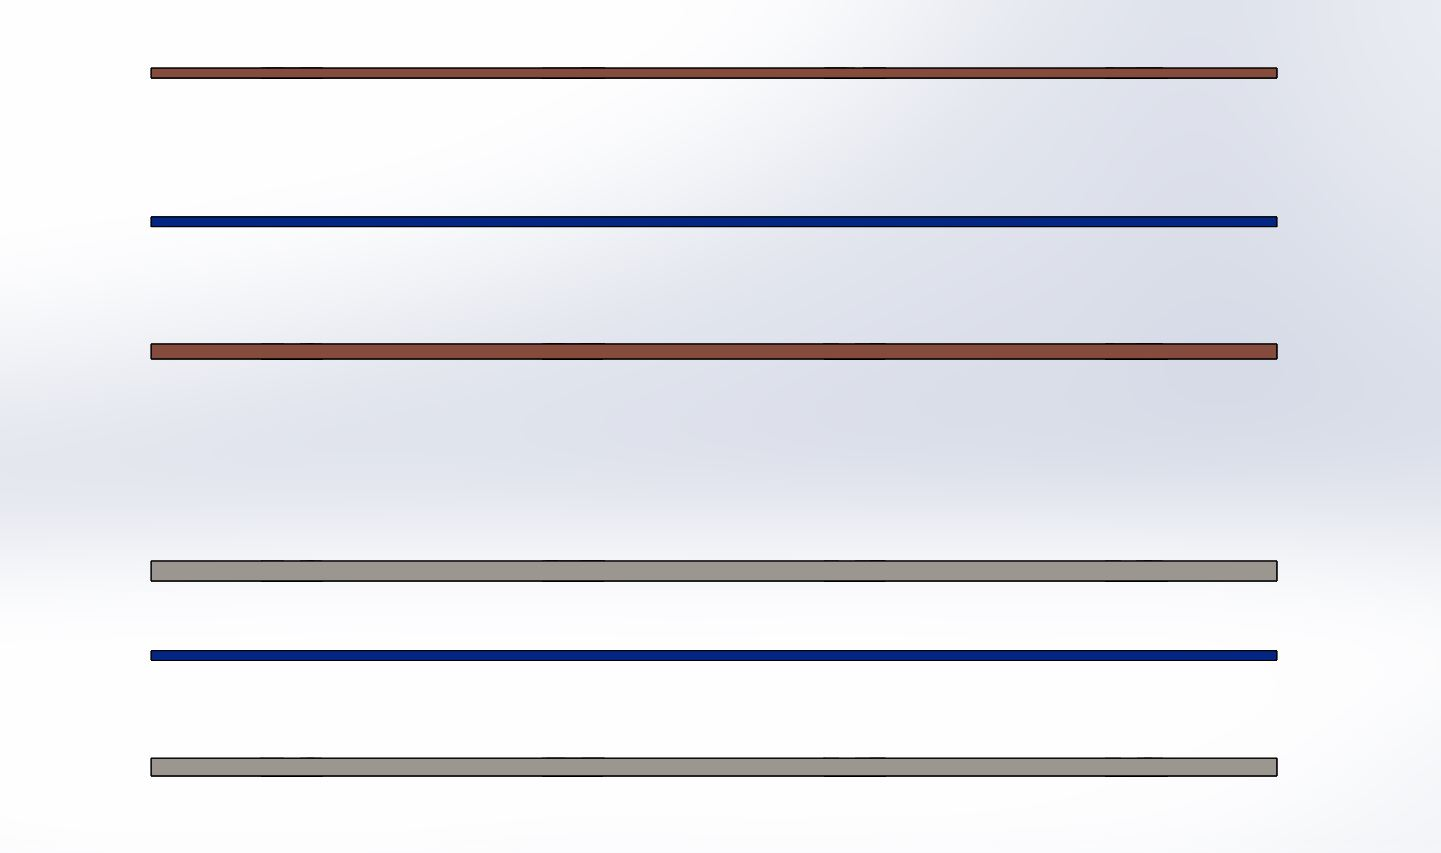
\includegraphics[width=\textwidth]{Petri_left}
  \caption{Right assembly view of proof-of-concept of `The Petri Dish'}
  \label{fig:petri_left}
\end{figure}

The petri dish design basically relies on placing many pieces of metal in close contact with each other to create a larger part. That is to say that if we needed a thick skin then this could be achieved by placing two or more thinner pieces of aluminum on top of each other. The benefit of this design is that we only need a single thin layer of aluminum that contains the crack. This layer can then be moved up or down to shift the crack into either the doubler or the skin or to a specific depth in the skin as required. The issue that was emergent with this design is that we need a non-lossy material that can be applied to the two layers brought into contact - this way the eddy-current does not see significant loss due to the air interface between aluminum layers. There are multiple ways to get around this with suggestions like metal embedded agarose gel, conductive tapes, or a simple salt-solution. In essence the interface-gel should have a conductivity on the same order as that of aluminum (the design can tolerate perhaps an order drop in conductivity). A design should be constrained so that the drop in power should be less than 3dB per assembled part [this can be calculated by $20 \log{\frac{<\rho>}{\rho_{Al}}}$, where $<\rho>$ is the conductivity of entire skin or doubler (the gel layers and the aluminum layers put together)] - the reason for a maximum drop of 3dB is that if we have both the doubler and the skin assemblies at 3dB then in total we would have a drop of 6dB or 50\% attenuation. 

In figures Fig.\ref{fig:petri_iso} and Fig.\ref{fig:petri_left} the gel is represented by the blue layer. The doubler sheets are the brown figures on the top, sandwiching the gel to create a thicker layer. The skin sheets are the grey sheets below, similarly sandwiching a layer of gel. There is no gel between the bottom doubler layer and the top skin layer as air is needed to accurately reflect the double-skin interface. Not pictured are the fasteners that would be in the assembly, and the machined cracks.
\clearpage

\section{Models and Evaluation}
Now that the alternatives for approaching different design aspects have been chosen, this section will determine the best of the alternatives by way of multi-criterion decision analysis. In this proposal we will be evaluating the designs using a weighted sum model where a number of alternatives are evaluated against each other. It is important to normalize the design features under consideration so that all the parameters have the same unit - for this purpose we are normalizing our design against Bombardier's calibration block, used by operator that we were shown. 

\subsection{\textsc{Constraints and Objectives}}

Constraints for the project were identified in the project requirements report previously submitted. These constraints and objectives are listed here for the benefit of the reader.

\textbf{Constraints:}
\begin{itemize}
\item Cost
\item Versatility
\item Regulatory compliance
\end{itemize}

Similarly the objectives of the proposed designs are also listed below for the reader. They are listed in order of priority (high to low) along with their normalized weights.

\textbf{Objectives:}
\begin{table}[h!]   
\begin{center}
    \begin{tabular}{ | l | c |}
    \hline
    Selection Criteria & Normalized Weight  \\ \hline
    Low Cost & 0.192    \\ \hline
    Reliability & 0.183    \\ \hline
    Manufacturability & 0.112    \\ \hline
    Ease of Use & 0.112    \\ \hline
    Portability & 0.112    \\ \hline
    Robustness & 0.103    \\ \hline
    Safety & 0.093    \\ \hline
    Traceability & 0.093    \\ \hline
	\end{tabular}
\caption{Table showing the normalized weight ascribed by the team to a given objective}
\label{norm}    
\end{center}
\end{table}

Due to the low priority the team gave to ergonomics (a score of 1.5 out of a maximum of 5) in the project requirements, it has been decided that the objective be dropped for the purposes of evaluation. As such ergonomics will not be a deciding factor between alternatives.


\subsection{\textsc{Weighted Sum Model}}
In general, with normalized features, the value of a specific design '$A$' can be given by: $$A^{WSM-score} = \sum_{j=1}^n {w_j \sum^{m_n}_{k=1} {u_{jk} a_{jk}}}$$ where $w_j$ is the normalized weight given to a particular objective '$j$' and $u_{jk}$ is the relative importance of a particular design feature '$k$' to the given objective, and $a_{jk}$ is the value of the design feature '$k$' evaluated against objective '$j$'. The total number of objectives is $n$ and the total number of features relating to that objective is $m_n$. The weights $w_j$ were decided in the project proposal and the normalized values are shown in Table. \ref{norm}. The weights $u_{jk}$ are shown in Table. \ref{table1} in the Appendix along with the features and their relative values $a_{jk}$.

\begin{table}[h!]   
\begin{center}
    \begin{tabular}{ | l | c |}
    \hline
    Proposed Design & Weighted Sum Minimization Score  \\ \hline
    The Staircase & 0.8597    \\ \hline
    The Petri Dish & 0.8642    \\ \hline
    The Hook & 0.9051    \\ \hline
	\end{tabular}
\caption{Table showing Proposed Designs and their Weighted Sum Minimization Scores}
\label{results}    
\end{center}
\end{table}


\subsection{\textsc{summary of final design}}
After optimization and decision analysis, Section 4 shows that the optimal design to be implemented is the `Staircase' design. The additional cost of the multiple cracks is countered by the higher reliability and ease of use.

While the team suggests and recommends the implementation of the `Staircase', the analysis shows that the other designs are still viable options. Should the client wish, the other designs may be expanded on and refined. Every design has room for additional improvements and functionality. They each make it possible to calibrate situations of two repair-doublers atop the skin. They all offer the use of different rivet/fastener types. The adjustments would be easy to incorporate, but the team feels this is especially true for the `Staircase' design.

\newpage
\section{Appendix}
%\addcontentsline{toc}{chapter}{Appendix}
\subsection{\textsc{Design Features and Objectives}}
% Please add the following required packages to your document preamble:
% \usepackage{graphicx}
% \usepackage[table,xcdraw]{xcolor}
% If you use beamer only pass "xcolor=table" option, i.e. \documentclass[xcolor=table]{beamer}
\begin{table}[h]
\centering
\caption{Table showing design features and scores as related to objectives}
\label{table1}
\resizebox{\textwidth}{!}{%
\begin{tabular}{rllll}
\multicolumn{1}{l}{\textbf{}}                  & \textbf{The Staircase}                                            & \textbf{The Petri Dish}                                           & \textbf{The Hook}                                                 & \textbf{Bombardier's CTS} \\ \cline{2-5} 
\multicolumn{1}{l}{\textbf{Cost}}              &                                                                   &                                                                   &                                                                   &                           \\ \cline{1-1}
Number of cracks                               & 42                                                                & 2                                                                 & 0                                                                 & 17                        \\
Number of processes (ignoring EDM)             & 3                                                                 & 3                                                                 & 4                                                                 & 3                         \\
\rowcolor[HTML]{C0C0C0} 
\textit{Normalized Cost of Crack}              & \multicolumn{1}{r}{\cellcolor[HTML]{C0C0C0}\textit{2.470588235}}  & \multicolumn{1}{r}{\cellcolor[HTML]{C0C0C0}\textit{0.1176470588}} & \multicolumn{1}{r}{\cellcolor[HTML]{C0C0C0}\textit{0}}            & \textit{}                 \\
\rowcolor[HTML]{C0C0C0} 
\textit{Number of Processes}                   & \multicolumn{1}{r}{\cellcolor[HTML]{C0C0C0}\textit{1}}            & \multicolumn{1}{r}{\cellcolor[HTML]{C0C0C0}\textit{1}} & \multicolumn{1}{r}{\cellcolor[HTML]{C0C0C0}\textit{1.333333333}}  & \textit{}                 \\
\multicolumn{1}{l}{}                           &                                                                   &                                                                   &                                                                   &                           \\
\multicolumn{1}{l}{\textbf{Safety}}            &                                                                   &                                                                   &                                                                   &                           \\ \cline{1-1}
Team Member 1                                  & 8                                                                 & 7                                                                 & 10                                                                & 8                         \\
Team Member 2                                  & 10                                                                & 7                                                                 & 7                                                                 & 10                        \\
Team Member 3                                  & 8                                                                 & 7                                                                 & 7                                                                 & 10                        \\
Team Member 4                                  & 9                                                                 & 6                                                                 & 9                                                                 & 10                        \\
Avg. Value                                     & 8.75                                                              & 6.75                                                              & 8.25                                                              & 9.333333333               \\
\rowcolor[HTML]{C0C0C0} 
\textit{Normalized and Reciprocal Safety Value}               & \multicolumn{1}{r}{\cellcolor[HTML]{C0C0C0}\textit{1.0667}}       & \multicolumn{1}{r}{\cellcolor[HTML]{C0C0C0}\textit{1.3827}} & \multicolumn{1}{r}{\cellcolor[HTML]{C0C0C0}\textit{1.1313}} & \textit{}                 \\
\multicolumn{1}{l}{}                           &                                                                   &                                                                   &                                                                   &                           \\
\multicolumn{1}{l}{\textbf{Portability}}       &                                                                   &                                                                   &                                                                   &                           \\ \cline{1-1}
Volume                                         & 20.46                                                             & 9.75                                                              & 3.41                                                              & 20                        \\
Surface Area                                   & 446                                                               & 95                                                                & 111.5                                                             & 400                       \\
Volume/Surface Area                            & 0.04587443946                                                     & 0.1026315789                                                      & 0.03058295964                                                     & 0.05                      \\
\rowcolor[HTML]{C0C0C0} 
\textit{Normalized Reciprocal Portability measure}         & \multicolumn{1}{r}{\cellcolor[HTML]{C0C0C0}\textit{1.090}} & \multicolumn{1}{r}{\cellcolor[HTML]{C0C0C0}\textit{0.4872}}  & \multicolumn{1}{r}{\cellcolor[HTML]{C0C0C0}\textit{1.6349}} & \textit{}                 \\
\multicolumn{1}{l}{}                           &                                                                   &                                                                   &                                                                   &                           \\
\multicolumn{1}{l}{\textbf{Ease of Use}}       &                                                                   &                                                                   &                                                                   &                           \\ \cline{1-1}
Number of individual parts                     & 8                                                                 & 13                                                                & 17                                                                & 8                         \\
Approximate Set-up time                        & 0                                                                 & 14                                                                 & 13.75                                                             &                           \\
\rowcolor[HTML]{C0C0C0} 
\textit{Normalized Part}                       & \multicolumn{1}{r}{\cellcolor[HTML]{C0C0C0}\textit{1}}            & \multicolumn{1}{r}{\cellcolor[HTML]{C0C0C0}\textit{1.625}}        & \multicolumn{1}{r}{\cellcolor[HTML]{C0C0C0}\textit{2.125}}        & \textit{}                 \\
\rowcolor[HTML]{C0C0C0} 
\textit{Normalized Set-Up Time}                & \multicolumn{1}{r}{\cellcolor[HTML]{C0C0C0}\textit{0}}            & \multicolumn{1}{r}{\cellcolor[HTML]{C0C0C0}\textit{1.4}}          & \multicolumn{1}{r}{\cellcolor[HTML]{C0C0C0}\textit{1.375}}        & \textit{}                 \\
\multicolumn{1}{l}{}                           &                                                                   &                                                                   &                                                                   &                           \\
\multicolumn{1}{l}{\textbf{Reliability}}       &                                                                   &                                                                   &                                                                   &                           \\ \cline{1-1}
\rowcolor[HTML]{C0C0C0} 
\textit{Reliability of Thickness Generation}   & \multicolumn{1}{r}{\cellcolor[HTML]{C0C0C0}\textit{0}}            & \multicolumn{1}{r}{\cellcolor[HTML]{C0C0C0}\textit{0.64}}        & \multicolumn{1}{r}{\cellcolor[HTML]{C0C0C0}\textit{1.33}}        & \textit{}                \\

\rowcolor[HTML]{C0C0C0} 
\textit{Probability of Error Propagation}   & \multicolumn{1}{r}{\cellcolor[HTML]{C0C0C0}\textit{0}}            & \multicolumn{1}{r}{\cellcolor[HTML]{C0C0C0}\textit{1}}        & \multicolumn{1}{r}{\cellcolor[HTML]{C0C0C0}\textit{0.4}}        & \textit{}                \\

\multicolumn{1}{l}{}                           &                                                                   &                                                                   &                                                                   &                           \\
\multicolumn{1}{l}{\textbf{Traceability}}      &                                                                   &                                                                   &                                                                   &                           \\ \cline{1-1}
\rowcolor[HTML]{C0C0C0} 
\textit{Binary Inverted Traceability Measure}           & \multicolumn{1}{r}{\cellcolor[HTML]{C0C0C0}\textit{0}}            & \multicolumn{1}{r}{\cellcolor[HTML]{C0C0C0}\textit{1}}            & \multicolumn{1}{r}{\cellcolor[HTML]{C0C0C0}\textit{0}}            &                          \\
\multicolumn{1}{l}{}                           &                                                                   &                                                                   &                                                                   &                           \\
\multicolumn{1}{l}{\textbf{Robustness}}        &                                                                   &                                                                   &                                                                   &                           \\ \cline{1-1}
Surface Area                                   & 446                                                               & 95                                                                & 111.5                                                             & 400                       \\
\rowcolor[HTML]{C0C0C0} 
\textit{Normalized Surface Area}               & \multicolumn{1}{r}{\cellcolor[HTML]{C0C0C0}\textit{1.115}}        & \multicolumn{1}{r}{\cellcolor[HTML]{C0C0C0}\textit{0.2375}}       & \multicolumn{1}{r}{\cellcolor[HTML]{C0C0C0}\textit{0.27875}}      & \textit{}                 \\
\multicolumn{1}{l}{}                           &                                                                   &                                                                   &                                                                   &                           \\
\multicolumn{1}{l}{\textbf{Manufacturability}} &                                                                   &                                                                   &                                                                   &                           \\ \cline{1-1}
Number of Manufacturing Processes used.    & 4                                                                 & 4                                                                 & 5                                                                 & 4                         \\
\rowcolor[HTML]{C0C0C0} 
\textit{Normalized Number of Processes}        & \multicolumn{1}{r}{\cellcolor[HTML]{C0C0C0}\textit{1}}            & \multicolumn{1}{r}{\cellcolor[HTML]{C0C0C0}\textit{1}}         & \multicolumn{1}{r}{\cellcolor[HTML]{C0C0C0}\textit{1.25}}         & \textit{}                
\end{tabular}
}
\end{table}

\newpage
\subsection{\textsc{Digital Precision EDM Quote}}


\begin{figure}[h!]
  \centering
  	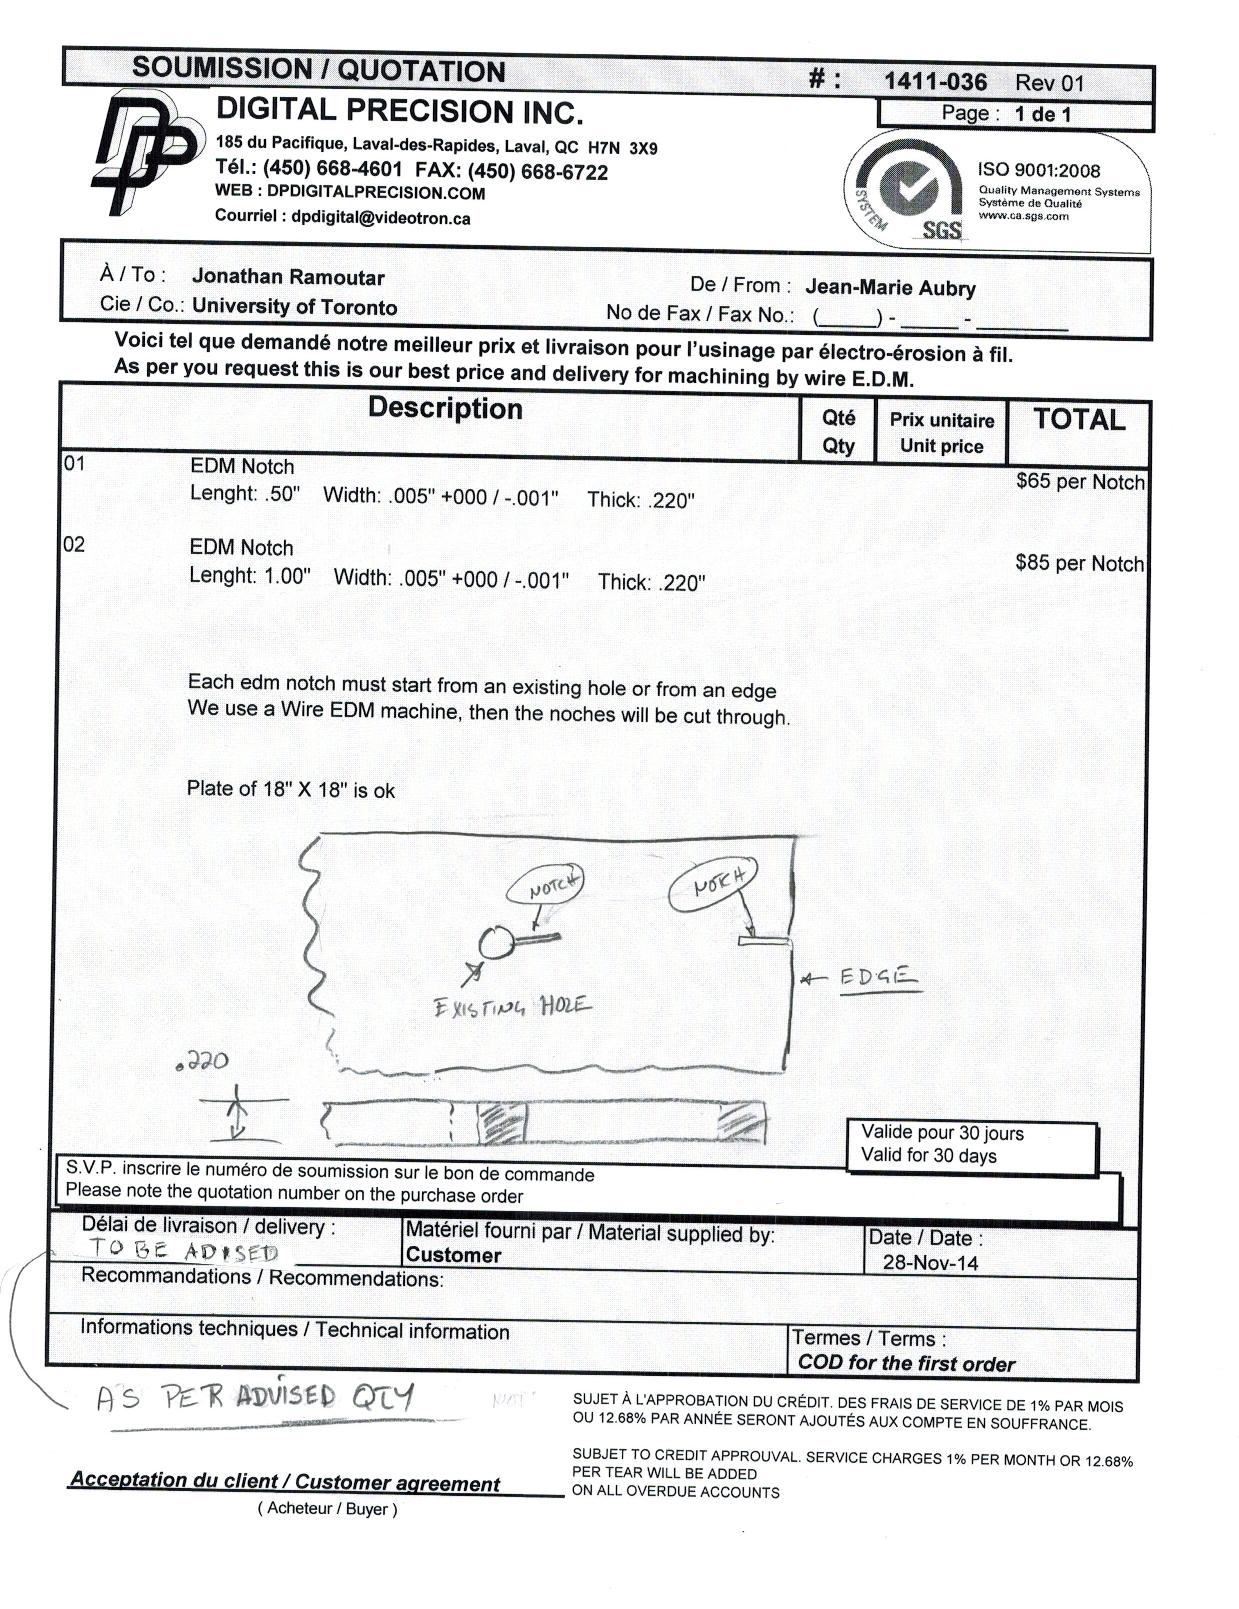
\includegraphics[width=0.95\textwidth]{quote.pdf}
  \label{fig:quote}
\end{figure}


%-------------------------------------------------------------------------------
% REFERENCES
%-------------------------------------------------------------------------------
\newpage
\section*{References}
\addcontentsline{toc}{section}{References}

\noindent
[1] MicroChemicals, 'Aluminium Etching', 2014. [Online]. Available: http://microchemicals. com/technical \_information/aluminium\_etching.pdf. [Accessed: 29- Nov- 2014].
\newline
\newline
\noindent
[2]K. Williams, K. Gupta and M. Wasilik, 'Etch rates for micromachining processing-part II', J. Microelectromech. Syst., vol. 12, no. 6, pp. 761-778, 2003.
\newline
\newline
\noindent
[3] Custompartnet.com, 'Machining Cost Estimator', 2014. [Online]. Available: http://www. custompartnet.com/estimate/machining/. [Accessed: 29- Nov- 2014].
\newline
\newline
\noindent
[4] Jobshop.com, 'Chemical Milling on JobShop.com', 2014. [Online]. Available: http://www. jobshop.com/techinfo/papers/chemmillpaper.shtml. [Accessed: 29- Nov- 2014].
\newline
\newline
\noindent


\end{document}

%-------------------------------------------------------------------------------
% SNIPPETS
%-------------------------------------------------------------------------------

%\begin{figure}[!ht]
%	\centering
%	\includegraphics[width=0.8\textwidth]{file_name}
%	\caption{}
%	\centering
%	\label{label:file_name}
%\end{figure}

%\begin{figure}[!ht]
%	\centering
%	\includegraphics[width=0.8\textwidth]{graph}
%	\caption{Blood pressure ranges and associated level of hypertension (American Heart Association, 2013).}
%	\centering
%	\label{label:graph}
%\end{figure}

%\begin{wrapfigure}{r}{0.30\textwidth}
%	\vspace{-40pt}
%	\begin{center}
%		\includegraphics[width=0.29\textwidth]{file_name}
%	\end{center}
%	\vspace{-20pt}
%	\caption{}
%	\label{label:file_name}
%\end{wrapfigure}

%\begin{wrapfigure}{r}{0.45\textwidth}
%	\begin{center}
%		\includegraphics[width=0.29\textwidth]{manometer}
%	\end{center}
%	\caption{Aneroid sphygmomanometer with stethoscope (Medicalexpo, 2012).}
%	\label{label:manometer}
%\end{wrapfigure}

%\begin{table}[!ht]\footnotesize
%	\centering
%	\begin{tabular}{cccccc}
%	\toprule
%	\multicolumn{2}{c} {Pearson's correlation test} & \multicolumn{4}{c} {Independent t-test} \\
%	\midrule	
%	\multicolumn{2}{c} {Gender} & \multicolumn{2}{c} {Activity level} & \multicolumn{2}{c} {Gender} \\
%	\midrule
%	Males & Females & 1st level & 6th level & Males & Females \\
%	\midrule
%	\multicolumn{2}{c} {BMI vs. SP} & \multicolumn{2}{c} {Systolic pressure} & \multicolumn{2}{c} {Systolic Pressure} \\
%	\multicolumn{2}{c} {BMI vs. DP} & \multicolumn{2}{c} {Diastolic pressure} & \multicolumn{2}{c} {Diastolic pressure} \\
%	\multicolumn{2}{c} {BMI vs. MAP} & \multicolumn{2}{c} {MAP} & \multicolumn{2}{c} {MAP} \\
%	\multicolumn{2}{c} {W:H ratio vs. SP} & \multicolumn{2}{c} {BMI} & \multicolumn{2}{c} {BMI} \\
%	\multicolumn{2}{c} {W:H ratio vs. DP} & \multicolumn{2}{c} {W:H ratio} & \multicolumn{2}{c} {W:H ratio} \\
%	\multicolumn{2}{c} {W:H ratio vs. MAP} & \multicolumn{2}{c} {\% Body fat} & \multicolumn{2}{c} {\% Body fat} \\
%	\multicolumn{2}{c} {} & \multicolumn{2}{c} {Height} & \multicolumn{2}{c} {Height} \\
%	\multicolumn{2}{c} {} & \multicolumn{2}{c} {Weight} & \multicolumn{2}{c} {Weight} \\
%	\multicolumn{2}{c} {} & \multicolumn{2}{c} {Heart rate} & \multicolumn{2}{c} {Heart rate} \\
%	\bottomrule
%	\end{tabular}
%	\caption{Parameters that were analysed and related statistical test performed for current study. BMI - body mass index; SP - systolic pressure; DP - diastolic pressure; MAP - mean arterial pressure; W:H ratio - waist to hip ratio.}
%	\label{label:tests}
%\end{table}
